The above equation can be expressed in the form 
\begin{align}
\vec{x}^T\vec{V}\vec{x}+2\vec{u}^T\vec{x}+f&=0
%\label{eq:solutions/40/7/2.2} 
\label{eq:solutions/40/7/eq1}
\intertext{Comparing equation we get}
    \vec{V}=\vec{V}^T&=\myvec{8 & 5 \\ 5 &-3}\label{eq:solutions/40/7/eqv}\\
    \vec{u}&=\myvec{-1 \\2 }\label{eq:solutions/40/7/equ}\\
    f&=-2\label{eq:solutions/40/7/eqfv}
\end{align}   
Expanding the Determinant of $\vec{V}$.
\begin{align}
    \Delta_{V} &= \begin{array}{|cc|}
8 &5\\5 & -3
\end{array}<0\label{eq:solutions/40/7/eq:hyp}
\end{align}
Hence from \eqref{eq:solutions/40/7/eq:hyp} given
equation represents the hyperbola
The characteristic equation of $\vec{V}$ is obtained by evaluating the determinant 
\begin{align}
       \begin{array}{|c|}
V-\lambda\vec{I}
\end{array}&=0\\
   \begin{array}{|cc|}
8-\lambda & 5 \\ 5 & -3-\lambda
\end{array}&=0\\
    \brak{8-\lambda}\brak{-3-\lambda}-25=0\\
    \lambda_{1}= \frac{5+\sqrt{221}}{2}\label{eq:solutions/40/7/eq:matrix_l1}\\
    \lambda_{2}= \frac{5-\sqrt{221}}{2}\label{eq:solutions/40/7/eq:matrix_l2}
\end{align}
The eigenvector $\vec{p}$ is defined as 
\begin{align}
    \vec{V}\vec{p}&=\lambda\vec{p}\\
    \implies (\vec{V}-\lambda\vec{I})\vec{p}&=0\label{eq:solutions/40/7/eq:7/eqev}
\end{align}
For $\lambda_1=\frac{5+\sqrt{221}}{2}$ ,
\begin{align}
    (\vec{V}-\lambda_1\vec{I})=\myvec{\frac{11-\sqrt{221}}{2} & 5 \\5 & \frac{-11-\sqrt{221}}{2}}
\end{align}
By row reduction , 
\begin{align}
    &\myvec{\frac{11-\sqrt{221}}{2} & 5 \\5 & \frac{-11-\sqrt{221}}{2}}\\
    %&\xleftrightarrow{\frac{R_1}{\frac{\sqrt{533}+2}{2}}}\\
    &\xleftrightarrow{R_1\leftarrow R_2}
    \myvec{\frac{-11-\sqrt{221}}{2} & 5 \\ \frac{11-\sqrt{221}}{2} & 5}\\
 &\xleftrightarrow{R_2\leftarrow R_2-\frac{11-\sqrt{221}}{10}R_{1}}
    \myvec{5 & \frac{-11-\sqrt{221}}{2} \\ 0& 0}\\
     &\xleftrightarrow{R_1\leftarrow R_1/5}
    \myvec{1 & \frac{-11-\sqrt{221}}{10} \\ 0& 0}
    \label{eq:solutions/40/7/eq:7/eqs1}
\end{align}
Subsituting equation \ref{eq:solutions/40/7/eq:7/eqs1} in equation \ref{eq:solutions/40/7/eq:7/eqev} we get
\begin{align}
        & \myvec{1 & \frac{-11-\sqrt{221}}{10} \\ 0& 0}\myvec{v_1 \\ v_2}=\myvec{0 \\ 0}\label{eq:solutions/40/7/eq:7/eqei1}
\end{align}
Where, $\vec{p}=\myvec{v_1\\v_2}$
Let $v_2=t$
\begin{align}
    v_1&=\frac{t(11+\sqrt{221})}{10}
\end{align}
Eigen vector $\vec{p_1}$ is given by
\begin{align}
    \vec{p_1}&=\myvec{\frac{t(11+\sqrt{221})}{10} \\ t}
\end{align}
Let $t=1$, we get
\begin{align}
        \vec{p_1}&=\myvec{\frac{11+\sqrt{221}}{10} \\1 }\label{eq:solutions/40/7/eq:es71/eqp1}
\end{align}
For $\lambda_2=\frac{5-\sqrt{221}}{2}$ ,
\begin{align}
    (\vec{V}-\lambda_2\vec{I})=\myvec{\frac{11+\sqrt{221}}{2} & 5 \\5 & \frac{-11+\sqrt{221}}{2}}
\end{align}
By row reduction , 
\begin{align}
     \myvec{\frac{11+\sqrt{221}}{2} & 5 \\5 & \frac{-11+\sqrt{221}}{2}}
    \xleftrightarrow{R_1\leftarrow R_2+ \frac{11-\sqrt{221}}{10}R_1}
     \myvec{\frac{11+\sqrt{221}}{2} &5\\ 0& 0}\\  
 \xleftrightarrow{R_1\leftarrow
 \frac{R_1}{\frac{11+\sqrt{221}}{10}}}
    \myvec{1 & \frac{10}{11+\sqrt{221}} \\ 0& 0}
    \label{eq:solutions/40/7/eq:es71/eqs2}
\end{align} 
Substiuting equation \ref{eq:solutions/40/7/eq:es71/eqs2} in equation \ref{eq:solutions/40/7/eq:7/eqev} we get 
\begin{align}
    &\myvec{1 & \frac{10}{11+\sqrt{221}} \\0 & 0}\myvec{v_1 \\ v_2}=\myvec{0 \\ 0}
%\label{eq:solutions/40/7/eq:es71/eqei1}
\end{align}
Where, $\vec{p}=\myvec{v_1\\v_2}$
Let $v_2=t$
\begin{align}
    v_1&=\frac{-t\brak{10}}{11+\sqrt{221}}
\end{align}
Eigen vector $\vec{p_2}$ is given by
\begin{align}
        \vec{p_2}&=\myvec{\frac{-t\brak{10}}{11+\sqrt{221}} \\ t}
\end{align}
Let $t=1$, we get 
\begin{align}
    \vec{p_2}&=\myvec{\frac{\brak{-10}}{11+\sqrt{221}} \\1 }\label{eq:solutions/40/7/eq:es71/eqp2}
\end{align}
By eigen decompostion $\vec{V}$ can be represented by
\begin{align}
    \vec{V}&=\vec{P}\vec{D}\vec{P}^T\label{eq:solutions/40/7/eq:es71/eqsubs}
\end{align}
where 
\begin{align}
        \vec{P}&=\myvec{\vec{p_1} & \vec{p_2}}\label{eq:solutions/40/7/eq:es71/eqp}\\
    \vec{D}&=\myvec{\lambda_1 & 0 \\0 & \lambda_2}\label{eq:solutions/40/7/eq:es71/eqD}
\end{align}
Substituting equations \ref{eq:solutions/40/7/eq:es71/eqp1}, \ref{eq:solutions/40/7/eq:es71/eqp2} in equation \ref{eq:solutions/40/7/eq:es71/eqp} we get 
\begin{align}
    \vec{P}&=\myvec{\frac{11+\sqrt{221}}{10} & \frac{-10}{11+\sqrt{221}} \\1 & 1}\label{eq:solutions/40/7/eq:es71/eqP}
\end{align}
Substituting equations \ref{eq:solutions/40/7/eq:matrix_l1}, \ref{eq:solutions/40/7/eq:matrix_l2} in \ref{eq:solutions/40/7/eq:es71/eqD} we get
\begin{align}
       \vec{D}&=\myvec{\frac{5+\sqrt{221}}{2} & 0\\0 & \frac{5-\sqrt{221}}{2}}\label{eq:solutions/40/7/eq:es71/eqDD}
\end{align}
Centre of the hyperbola is given by 
\begin{align}
    \vec{c}&=-\vec{V}^{-1}\vec{u}\\
    \implies\vec{c}&=-\myvec{\frac{3}{49}&\frac{5}{49}\\\frac{5}{49}&\frac{-8}{49}}\myvec{-1 \\ 2}\\
    \implies\vec{c}&=\myvec{\frac{-3}{49}&\frac{-5}{49}\\\frac{-5}{49}&\frac{8}{49}}\myvec{-1 \\ 2}\\
    \implies\vec{c}&=\myvec{\frac{-1}{7}\\\frac{3}{7}}
\end{align}
Since,
\begin{align}
    \vec{u}^T\vec{V}^{-1}\vec{u}-f = 1 > 0\label{eq:solutions/40/7/eq:es71/cond}
\end{align} 
there isn't a need to swap axes
In hyperbola,
\begin{align}
axes=
\begin{cases}
\sqrt{\frac{\vec{u}^T\vec{V}^{-1}\vec{u}-f}{\lambda_1}}\\ \sqrt{\frac{f-\vec{u}^T\vec{V}^{-1}\vec{u}}{\lambda_2}}
\end{cases}
\end{align}
From above equations we can say that,
\begin{align}
\sqrt{\frac{\vec{u}^T\vec{V}^{-1}\vec{u}-f}{\lambda_1}}=\sqrt{ \frac{2}{5+\sqrt{221}}}\\
\sqrt{\frac{f-\vec{u}^T\vec{V}^{-1}\vec{u}}{\lambda_2}}=\sqrt{ \frac{2}{5-\sqrt{221}}}
\end{align}
Now we have,
\begin{align}
    \vec{y}^T\vec{D}\vec{y}&=\vec{u}^T\vec{V}^{-1}\vec{u}-f\label{eq:solutions/40/7/eq:es71/fi}
\end{align}
where ,
\begin{align}
    \vec{y}&=\vec{P}^T(\vec{x}-\vec{c})
\end{align}
To get $\vec{y}$,
\begin{align}
\vec{y}&=\vec{P}^T\vec{x}-\vec{P}^T\vec{c}\\
    \vec{y}&= \myvec{\frac{11+\sqrt{221}}{10} & 1 \\ \frac{-10}{11+\sqrt{221}} & 1}\vec{x}-\myvec{\frac{11+\sqrt{221}}{10} & 1 \\ \frac{-10}{11+\sqrt{221}} & 1}\myvec{\frac{-1}{7}\\\frac{3}{7}}\\
    \vec{y}&=\myvec{\frac{11+\sqrt{221}}{10} & 1 \\ \frac{-10}{11+\sqrt{221}} & 1}\vec{x}-\myvec{\frac{-11-\sqrt{221}}{70}+\frac{3}{7} \\ \frac{10}{(7)11+(7)\sqrt{221}}+\frac{3}{7}}
\end{align}
Subsituting the eqauations \eqref{eq:solutions/40/7/eq:es71/cond}, \eqref{eq:solutions/40/7/eq:es71/eqDD} in equation \eqref{eq:solutions/40/7/eq:es71/fi}
\begin{align}
   \implies\vec{y}^T\myvec{\frac{5+\sqrt{221}}{2} & 0 \\0 & \frac{5-\sqrt{221}}{2}}\vec{y}+2&=0
\end{align}
{Asymptotes of hyperbola}
Equation of a hyperbola and the combined equation of the Asymptotes differ only in the constant term.
\begin{align}
 8x^2+10xy-3y^2-2x+4y+K=0   
\end{align}
The above equation can be expressed in the form 
\begin{align}
\vec{x}^T\vec{V}\vec{x}+2\vec{u}^T\vec{x}+f&=0
%\label{eq:solutions/40/7/2.2} 
%\label{eq:solutions/40/7/eq1}
\intertext{Comparing equation we get}
    \vec{V}=\vec{V}^T&=\myvec{8 & 5 \\ 5 &-3}\label{eq:solutions/40/7/es1/eqv}\\
    \vec{u}&=\myvec{-1 \\2 }\label{eq:solutions/40/7/eq:equ}\\
    f&=K\label{eq:solutions/40/7/eq:es1/eqfv}
\end{align}   
\begin{align}
\Delta&=\begin{array}{|ccc|}
8 & 5 & -1\\ 5& -3 & 2\\ -1 & 2 & K
\end{array}\\
\implies K&=-1
\end{align}
Similar way expanding the Determinant of $\vec{V}$.
\begin{align}
    \Delta_{V} &= \begin{array}{|cc|}
8 &5\\5 & -3
\end{array}<0\label{eq:solutions/40/7/eq:es/17/hyp}
\end{align}
From \eqref{eq:solutions/40/7/eq:es/17/hyp} we could say that the given equation represents two straight lines
Let the equations of lines be,
\begin{align}
	\brak{\vec{n_1}^T \vec{x} - c_1}\brak{\vec{n_1}^T \vec{x} - c_1} =
        \vec{x}^{T}\vec{Vx} + 2\vec{u}^{T}\vec{x} + f=0\label{eq:solutions/40/7/eq:eql7/03}
\end{align}
\begin{align}
\brak{\vec{n_1}^T\vec{x}-c_1}\brak{\vec{n_2}^T\vec{x}-c_2}
&=\vec{x}^T\myvec{8 & 5 \\ 5 & -3}\vec{x}\notag\\
+2\myvec{-1 & 2}\vec{x}-1\label{eq:solutions/40/7/equate}\\
    \vec{n_1}*\vec{n_2} = \myvec{a\\2b\\c} &= \myvec{8\\10\\-3}\label{eq:solutions/40/7/conv}\\
    c_2\vec{n_1}+c_1\vec{n_2}&=-2\myvec{-1\\2}\label{eq:solutions/40/7/eq17/c1c2}\\
    c_1c_2&=-1
\end{align}
The slopes of the lines are given by the roots of the polynomial 
\begin{align}
    &cm^2+2bm+a=0\label{eq:solutions/40/7/e}\\
    \implies m_i&=\frac{-b\pm{\sqrt{-\Delta_{V}}}}{c}\\
    \vec{n_i}&=k\myvec{-m_i\\1}
\end{align}
Substituting the given data in above equations \eqref{eq:solutions/40/7/e} we get,
\begin{align}
    &-3m^2+10m+8=0\\
    m_1&=4,  m_2=\frac{-2}{3}\\
   &= \vec{n_1}=\myvec{-4\\ 1}, \vec{n_2}=\myvec{-2\\-3} \label{eq:solutions/40/7/eq:normal1}
\intertext{We know that,}
& \vec{n_1}\ast \vec{n_2} = \myvec{a\\2b\\c} \label{eq:solutions/40/7/eq:conv1}
\end{align}
Verification using Toeplitz matrix, From equation \eqref{eq:solutions/40/7/eq:normal1}
\begin{align}
    \vec{n_1}=\myvec{-4&0\\1&-4\\0&-1}
    \vec{n_2}=\myvec{-2\\-3}\label{eq:solutions/40/7/eq:conv2}\\
\implies \myvec{-4&0\\1&-4\\0&1}\myvec{0\\ -1} = \myvec{8\\10\\-3} = \myvec{a\\2b\\c}\label{eq:solutions/40/7/eq:conv3}
\end{align}
$\implies$ Equation \eqref{eq:solutions/40/7/eq:normal1} satisfies \eqref{eq:solutions/40/7/eq:conv1}\\
$c_1$ and $c_2$ can be obtained as,
\begin{align}
\myvec{\vec{n_1} & \vec{n_2}}\myvec{c_2\\c_1}&=-2\vec{u} \label{eq:solutions/40/7/eq:aug1}
\end{align}
Substituting \eqref{eq:solutions/40/7/eq:normal1} in \eqref{eq:solutions/40/7/eq:aug1}, the augmented matrix is,
\begin{align}
\myvec{-4 & -2 & -2 \\ 1 & -3 & 4}
\xleftrightarrow[R_2\leftarrow R_2-R_1]{R_1\leftarrow -R_1/4}
\myvec{1 &\frac{1}{2} &\frac{1}{2} \\ 0 & -\frac{7}{2} & \frac{7}{2}} \label{eq:solutions/40/7/eq:aug5}\\
\xleftrightarrow[R_1\leftarrow R_1-\frac{1}{2}R_2]{R_2\leftarrow -\frac{2}{7}R_2}
\myvec{1 &0 &1 \\ 0& 1 & -1} \label{eq:solutions/40/7/eq:aug2}\\
\implies c_1 = 1, c_2=-1 \label{eq:solutions/40/7/eq:const1}
\end{align}
Equations \eqref{eq:solutions/40/7/eq:eql7/03}, can be modified as,from \eqref{eq:solutions/40/7/eq:normal1} and \eqref{eq:solutions/40/7/eq:const1} in we get,
\begin{align}
    \myvec{-4 & 1}\vec{x}&=1\\
    \myvec{-2 & -3}\vec{x}&=-1
\end{align}
\begin{multline}
\implies \brak{-4x+y-1}\brak{-2x-3y+1}= 0\\
\implies \boxed{\brak{4x-y+1}\brak{2x+3y-1} = 0} \label{eq:solutions/40/7/eq:line1}
\end{multline}
The angle between the lines can be expressed as, 
\begin{align}
	\vec{n_1}=\myvec{-4\\1} , \quad \vec{n_2}=\myvec{-2\\-3}\\
	\cos\theta=\frac{\vec{n_1}^T\vec{n_2}}{\norm{\vec{n_1}}\norm{\vec{n_2}}} \\
	\implies \quad \theta=\cos^{-1}({\frac{0}{\sqrt{221}}}) = 90\degree.
\end{align}
{Equation of Asymptotes: }
The characteristic equation of $\vec{V}$ is obtained by evaluating the determinant \eqref{eq:solutions/40/7/es1/eqv}
\begin{align}
       \begin{array}{|c|}
V-\lambda\vec{I}
\end{array}&=0\\
   \begin{array}{|cc|}
8-\lambda & 5 \\ 5 & -3-\lambda
\end{array}&=0\\
    \brak{8-\lambda}\brak{-3-\lambda}-25=0\\
    \lambda_{1}= \frac{5+\sqrt{221}}{2}\\
    \lambda_{2}= \frac{5-\sqrt{221}}{2}
\end{align}
The eigenvector $\vec{p}$ is defined as 
\begin{align}
    \vec{V}\vec{p}&=\lambda\vec{p}\\
    \implies (\vec{V}-\lambda\vec{I})\vec{p}&=0\label{eq:solutions/40/7/eq:es/2701}
\end{align}
For $\lambda_1=\frac{5+\sqrt{221}}{2}$ ,
\begin{align}
    (\vec{V}-\lambda_1\vec{I})=\myvec{\frac{11-\sqrt{221}}{2} & 5 \\5 & \frac{-11-\sqrt{221}}{2}}
\end{align}
By row reduction , 
\begin{align}
    &\myvec{\frac{11-\sqrt{221}}{2} & 5 \\5 & \frac{-11-\sqrt{221}}{2}}\\
    %&\xleftrightarrow{\frac{R_1}{\frac{\sqrt{533}+2}{2}}}\\
    &\xleftrightarrow{R_1\leftarrow R_2}
    \myvec{\frac{-11-\sqrt{221}}{2} & 5 \\ \frac{11-\sqrt{221}}{2} & 5}\\
 &\xleftrightarrow{R_2\leftarrow R_2-\frac{11-\sqrt{221}}{10}R_{1}}
    \myvec{5 & \frac{-11-\sqrt{221}}{2} \\ 0& 0}\\
     &\xleftrightarrow{R_1\leftarrow R_1/5}
    \myvec{1 & \frac{-11-\sqrt{221}}{10} \\ 0& 0}
    \label{eq:solutions/40/7/eq:es27/02}
\end{align}
Subsituting equation \ref{eq:solutions/40/7/eq:es27/02} in equation \ref{eq:solutions/40/7/eq:es/2701} we get
\begin{align}
        & \myvec{1 & \frac{-11-\sqrt{221}}{10} \\ 0& 0}\myvec{v_1 \\ v_2}=\myvec{0 \\ 0}\label{eq:solutions/40/7/eq:es27/eqei1}
\end{align}
Where, $\vec{p}=\myvec{v_1\\v_2}$
Let $v_2=t$
\begin{align}
    v_1&=\frac{t(11+\sqrt{221})}{10}
\end{align}
Eigen vector $\vec{p_1}$ is given by
\begin{align}
    \vec{p_1}&=\myvec{\frac{t(11+\sqrt{221})}{10} \\ t}
\end{align}
Let $t=1$, we get
\begin{align}
        \vec{p_1}&=\myvec{\frac{11+\sqrt{221}}{10} \\1 }\label{eq:solutions/40/7/eq:es27/eqp1}
\end{align}
For $\lambda_2=\frac{5-\sqrt{221}}{2}$ ,
\begin{align}
    (\vec{V}-\lambda_2\vec{I})=\myvec{\frac{11+\sqrt{221}}{2} & 5 \\5 & \frac{-11+\sqrt{221}}{2}}
\end{align}
By row reduction , 
\begin{align}
    \myvec{\frac{11+\sqrt{221}}{2} & 5 \\5 & \frac{-11+\sqrt{221}}{2}}
    \xleftrightarrow{R_1\leftarrow R_2+ \frac{11-\sqrt{221}}{10}R_1}
     \myvec{\frac{11+\sqrt{221}}{2} &5\\ 0& 0}\\  
 \xleftrightarrow{R_1\leftarrow
 \frac{R_1}{\frac{11+\sqrt{221}}{10}}}
    \myvec{1 & \frac{10}{11+\sqrt{221}} \\ 0& 0}
    \label{eq:solutions/40/7/eq:es27eqs02}
\end{align}
Subsituting equation \ref{eq:solutions/40/7/eq:es27eqs02} in equation \ref{eq:solutions/40/7/eq:es/2701} we get 
\begin{align}
    &\myvec{1 & \frac{10}{11+\sqrt{221}} \\0 & 0}\myvec{v_1 \\ v_2}=\myvec{0 \\ 0}
%\label{eq:solutions/40/7/eq:es27/eqei1}
\end{align}
Where, $\vec{p}=\myvec{v_1\\v_2}$
Let $v_2=t$
\begin{align}
    v_1&=\frac{-t\brak{10}}{11+\sqrt{221}}
\end{align}
Eigen vector $\vec{p_2}$ is given by
\begin{align}
        \vec{p_2}&=\myvec{\frac{-t\brak{10}}{11+\sqrt{221}} \\ t}
\end{align}
Let $t=1$, we get 
\begin{align}
    \vec{p_2}&=\myvec{\frac{\brak{-10}}{11+\sqrt{221}} \\1 }\label{eq:solutions/40/7/eq:es27/eqp2}
\end{align}
By eigen decompostion $\vec{V}$ can be represented by
\begin{align}
    \vec{V}&=\vec{P}\vec{D}\vec{P}^T\label{eq:solutions/40/7/eq:es27/eqsubs}
\end{align}
where 
\begin{align}
        \vec{P}&=\myvec{\vec{p_1} & \vec{p_2}}\label{eq:solutions/40/7/eq:es27/eqp}\\
    \vec{D}&=\myvec{\lambda_1 & 0 \\0 & \lambda_2}\label{eq:solutions/40/7/eq:es27/eqD}
\end{align}
Substituting equations \ref{eq:solutions/40/7/eq:es27/eqp1}, \ref{eq:solutions/40/7/eq:es27/eqp2} in equation \ref{eq:solutions/40/7/eq:es27/eqp} we get 
\begin{align}
    \vec{P}&=\myvec{\frac{11+\sqrt{221}}{10} & \frac{-10}{11+\sqrt{221}} \\1 & 1}\label{eq:solutions/40/7/eq:es27/eqP}
\end{align}
\begin{align}
       \vec{D}&=\myvec{\frac{5+\sqrt{221}}{2} & 0\\0 & \frac{5-\sqrt{221}}{2}}\label{eq:solutions/40/7/eq:es27/eqDD}
\end{align}
Centre of the hyperbola is given by 
\begin{align}
    \vec{c}&=-\vec{V}^{-1}\vec{u}\\
    \implies\vec{c}&=-\myvec{\frac{3}{49}&\frac{5}{49}\\\frac{5}{49}&\frac{-8}{49}}\myvec{-1 \\ 2}\\
    \implies\vec{c}&=\myvec{\frac{-3}{49}&\frac{-5}{49}\\\frac{-5}{49}&\frac{8}{49}}\myvec{-1 \\ 2}\\
    \implies\vec{c}&=\myvec{\frac{-1}{7}\\\frac{3}{7}}
\end{align}
Since,
\begin{align}
    \vec{u}^T\vec{V}^{-1}\vec{u}-f = 0\label{eq:solutions/40/7/eq:es27/cond}
\end{align} 
Now,
\begin{align}
    \vec{y}^T\vec{D}\vec{y}&=\vec{u}^T\vec{V}^{-1}\vec{u}-f\label{eq:solutions/40/7/eq:es27/fi}
\end{align}
where ,
\begin{align}
    \vec{y}&=\vec{P}^T(\vec{x}-\vec{c})
\end{align}
To get $\vec{y}$,
\begin{align}
\vec{y}&=\vec{P}^T\vec{x}-\vec{P}^T\vec{c}\\
    \vec{y}&= \myvec{\frac{11+\sqrt{221}}{10} & 1 \\ \frac{-10}{11+\sqrt{221}} & 1}\vec{x}-\myvec{\frac{11+\sqrt{221}}{10} & 1 \\ \frac{-10}{11+\sqrt{221}} & 1}\myvec{\frac{-1}{7}\\\frac{3}{7}}\\
    \vec{y}&=\myvec{\frac{11+\sqrt{221}}{10} & 1 \\ \frac{-10}{11+\sqrt{221}} & 1}\vec{x}-\myvec{\frac{-11-\sqrt{221}}{70}+\frac{3}{7} \\ \frac{10}{(7)11+(7)\sqrt{221}}+\frac{3}{7}}
\end{align}
Subsituting the eqauations \eqref{eq:solutions/40/7/eq:es27/cond}, \eqref{eq:solutions/40/7/eq:es27/eqDD} in equation \eqref{eq:solutions/40/7/eq:es27/fi}
Equation of asymptotes is
\begin{align}
    \implies \vec{y}^T\myvec{\frac{5+\sqrt{221}}{2} & 0 \\0 & \frac{5-\sqrt{221}}{2}}\vec{y}+1&=0
\end{align}
And the Equations of Conjugate hyperbola is 2(Equation of Asymptotes)- Equation of hyperbola. 
\begin{align}
    \implies \vec{y}^T\myvec{\frac{5+\sqrt{221}}{2} & 0 \\0 & \frac{5-\sqrt{221}}{2}}\vec{y}&=0
\end{align}
\begin{figure}[h]
    \centering
    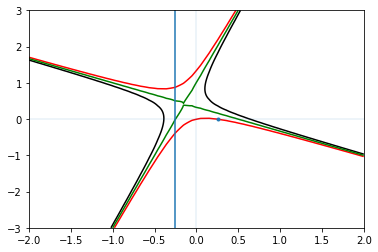
\includegraphics[width=\columnwidth]{./solutions/40/7/figs/A7_4.png}
    \caption{Hyperbola with assymptotes and its conjugate}
    \label{eq:solutions/40/7/Fig :1}
\end{figure}
